\documentclass{article}



\usepackage{fullpage}
\usepackage{nopageno}
\usepackage{amsmath}
\usepackage{amsfonts}
\usepackage{graphicx}
\usepackage{framed}
\usepackage{xcolor}

\definecolor{dark_red}{rgb}{0.5,0.0,0.0}
\definecolor{dark_green}{rgb}{0.0,0.5,0.0}
\definecolor{dark_blue}{rgb}{0.0,0.0,0.5}
\definecolor{blue}{rgb}{0.0,0.0,1.0}

\newcommand{\dr}[1]{\textcolor{dark_red}{#1}}
\newcommand{\dg}[1]{\textcolor{dark_green}{#1}}
\newcommand{\db}[1]{\textcolor{dark_blue}{#1}}
\newcommand{\blue}[1]{\textcolor{blue}{#1}}


\begin{document}

\section*{Parabolas}

\begin{tabular}{cc}
\parbox{0.5\textwidth}{
The general parabola has an equation with the form:
\[y = a(x + p)^2 + q\] 
where \(a\), \(p\), and \(q\) are fixed constants. \\
The shape of this parabola is a ``cup" as seen to the right. The {\bf turning point} of a parabola is the apex of the parabola, the point at which the value of \(y\) transitions, as \(x\) increases, from a state of decreasing to increasing (\(a > 0\)), or from increasing to decreasing (\(a < 0\)). The turning point will always be located at the point \((-p, q)\). \\
The basic parabola has the equation 
\[y = x^2\]
This parabola is the red curves on the right. In the case of \(y = x^2\), the turning point is \((0, 0)\). \\
Stretching this parabola vertically by a scale of \(a\) gives the equation:
\[y/a = x^2 \iff y = a x^2\] 
These parabolas are the green curves on the right. The parabola is vertically flipped if \(a < 0\) as seen in the lower image on the right. \\
Shifting the stretched parabola through a displacement of \(\langle -p, q \rangle\) gives the equation:
\[y - q = a(x - (-p))^2 \iff y = a(x + p)^2 + q\]
These parabolas are the blue curves on the right. The turning point is \((-p, q)\).
} & \parbox{0.5\textwidth}{
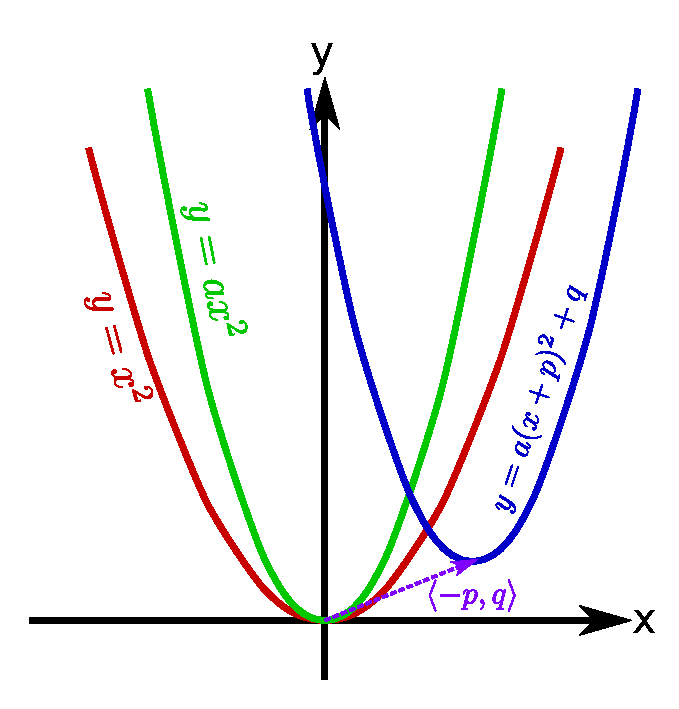
\includegraphics[width = 0.5\textwidth]{parabolas_1} \\ 
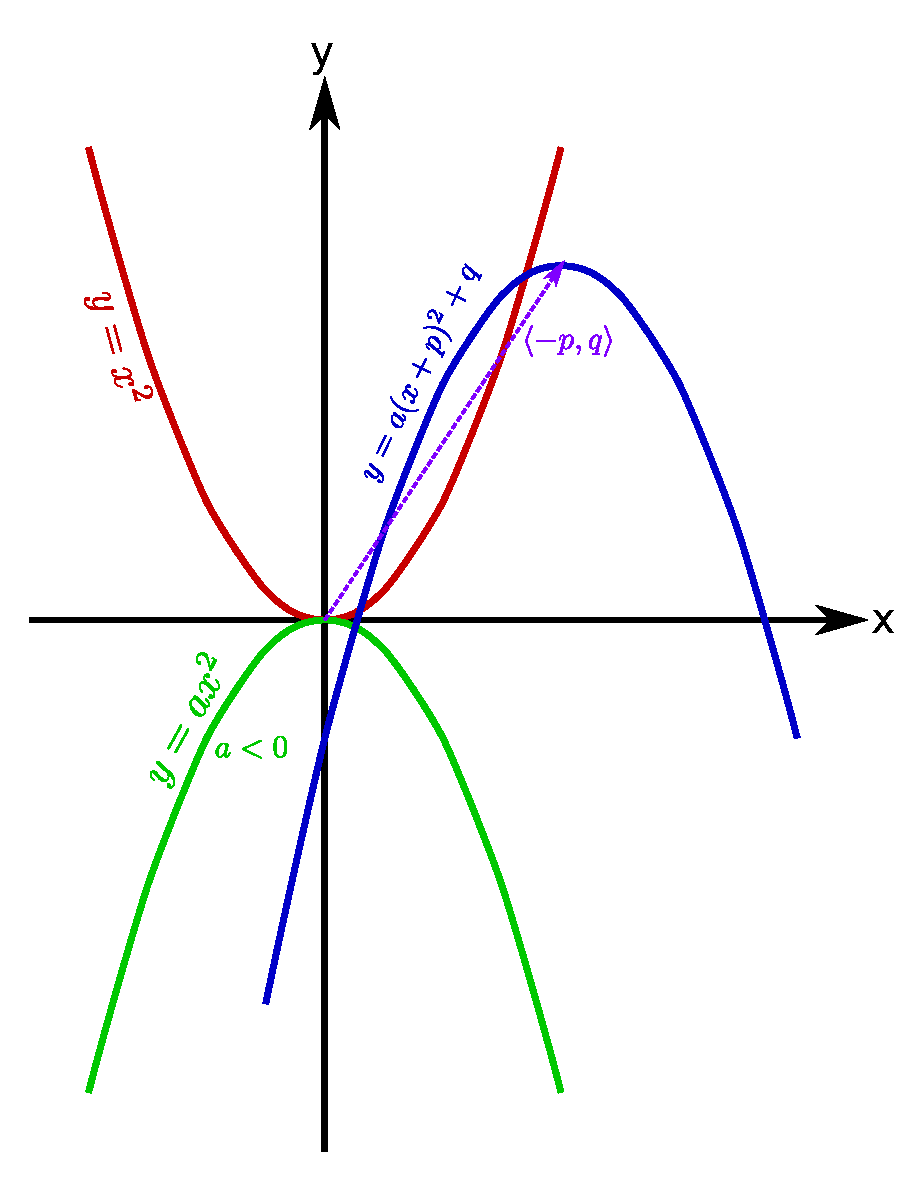
\includegraphics[width = 0.5\textwidth]{parabolas_2}
}
\end{tabular}

Every equation of the form 
\[y = ax^2 + bx + c\]
graphs a parabola. Completing the square is used to convert the equation \(y = ax^2 + bx + c\) to the form:
\[y = a(x + p)^2 + q\] 
Staring from 
\[y = ax^2 + bx + c\]
Firstly, \(a\) is factored from the first two terms to give:
\[y = a(x^2 + \frac{b}{a}x) + c\]
Next, the square of a binomial is completed by adding and subtracting the final term:
\[y = a((x^2 + 2\frac{b}{2a}x + (\frac{b}{2a})^2) - (\frac{b}{2a})^2) + c\]
Lastly collapsing the square expression \(x^2 + 2\frac{b}{2a}x + (\frac{b}{2a})^2\) to \((x + \frac{b}{2a})^2\) gives:
\[y = a(x + \frac{b}{2a})^2 + (c - \frac{b^2}{4a})\]
Several examples are given below:


\textbf{Examples:}
\begin{itemize}
%%%%%%%%%%%%%%
\item Consider the quadratic equation:
\dg{\[y = x^2 + 14x + 40\]}
\begin{align*}
y = & x^2 + 14x + 40 
= ((x^2 + 2 \cdot 7 \cdot x + 7^2) - 49) + 40 
= (x + 7)^2 - 9
\end{align*}
Therefore:
\blue{\[y = (x + 7)^2 - 9\]}
The parabola's turning point is \((-7, -9)\)
%%%%%%%%%%%%%%
\item Consider the quadratic equation:
\dg{\[y = 2x^2 - 20x + 48\]}
\begin{align*}
y = & 2x^2 - 20x + 48 
= 2(x^2 - 10x) + 48 
= 2((x^2 + 2 \cdot (-5) \cdot x + (-5)^2) - 25) + 48 \\
= & 2(x - 5)^2 - 2
\end{align*}
Therefore:
\blue{\[y = 2(x - 5)^2 - 2\]}
The parabola's turning point is \((5, -2)\)
%%%%%%%%%%%%%%
\item Consider the quadratic equation:
\dg{\[y = -x^2 - 6x - 5\]}
\begin{align*}
y = & -x^2 - 6x - 5 
= -(x^2 + 6x) - 5 
= -((x^2 + 2 \cdot 3 \cdot x + 3^2) - 9) - 5 \\
= & -(x + 3)^2 + 4
\end{align*}
Therefore: 
\blue{\[y = -(x + 3)^2 + 4\]}
The parabola's turning point is \((-3, 4)\)
%%%%%%%%%%%%%%
\item Consider the quadratic equation:
\dg{\[y = \frac{1}{3}x^2 + \frac{2}{3}x - \frac{8}{3}\]}
\begin{align*}
y = & \frac{1}{3}x^2 + \frac{2}{3}x - \frac{8}{3}  
= \frac{1}{3}(x^2 + 2x) - \frac{8}{3} 
= \frac{1}{3}((x^2 + 2 \cdot 1 \cdot x + 1^2) - 1) - \frac{8}{3} \\
= & \frac{1}{3}(x + 1)^2 - 3
\end{align*}
Therefore:
\blue{\[y = \frac{1}{3}(x + 1)^2 - 3\]}
The parabola's turning point is \((-1, -3)\)
%%%%%%%%%%%%%%
\item Consider the quadratic equation:
\dg{\[y = 5x^2 - 20x + 20\]}
\begin{align*}
y = & 5x^2 - 20x + 20 
= 5(x^2 - 4x) + 20 
= 5((x^2 + 2 \cdot (-2) \cdot x + (-2)^2) - 4) + 20 \\
= & 5(x - 2)^2
\end{align*}
Therefore:
\blue{\[y = 5(x - 2)^2\]}
The parabola's turning point is \((2, 0)\)
%%%%%%%%%%%%%%
\item Consider the quadratic equation:
\dg{\[y = -4x^2 + 16x - 32\]}
\begin{align*}
y = & -4x^2 + 16x - 32  
= -4(x^2 - 4x) - 32 
= -4((x^2 + 2 \cdot (-2) \cdot x + (-2)^2) - 4) - 32 \\ 
= & -4(x - 2)^2 - 16
\end{align*}
Therefore:
\blue{\[y = -4(x - 2)^2 - 16\]}
The parabola's turning point is \((2, -16)\) 
%%%%%%%%%%%%%%
\item Consider the quadratic equation:
\dg{\[y = \frac{1}{5}x^2 + \frac{6}{5}x + 2\]}
\begin{align*}
y = & \frac{1}{5}x^2 + \frac{6}{5}x + 2 
= \frac{1}{5}(x^2 + 6x) + 2 
= \frac{1}{5}((x^2 + 2 \cdot 3 \cdot x + 3^2) - 9) + 2 \\
= & \frac{1}{5}(x + 3)^2 + \frac{1}{5}
\end{align*}
Therefore:
\blue{\[y = \frac{1}{5}(x + 3)^2 + \frac{1}{5}\]}
The parabola's turning point is \((-3, 1/5)\)
%%%%%%%%%%%%%%
\item Consider the quadratic equation:
\dg{\[y = -2x^2 + 24x - 64\]}
\begin{align*}
y = & -2x^2 + 24x - 64 
= -2(x^2 - 12x) - 64 
= -2((x^2 + 2 \cdot (-6) \cdot x + (-6)^2) - 36) - 64 \\
= & -2(x - 6)^2 + 8
\end{align*}
Therefore:
\blue{\[y = -2(x - 6)^2 + 8\]}
The parabola's turning point is \((6, 8)\)
%%%%%%%%%%%%%%
\item Consider the quadratic equation:
\dg{\[y = 9x^2 - 6x - 35\]}
\begin{align*}
y = & 9x^2 - 6x - 35   
= 9(x^2 - \frac{2}{3}x) - 35 
= 9((x^2 + 2 \cdot (-\frac{1}{3}) \cdot x + (-\frac{1}{3})^2) - \frac{1}{9}) - 35 \\
= & 9(x - \frac{1}{3})^2 - 36
\end{align*}
Therefore:
\blue{\[y = 9(x - \frac{1}{3})^2 - 36\]}
The parabola's turning point is \((1/3, -36)\)
%%%%%%%%%%%%%%
\item Consider the quadratic equation:
\dg{\[y = 8x^2 + 40x + 32\]}
\begin{align*}
y = & 8x^2 + 40x + 32 
= 8(x^2 + 5x) + 32 
= 8((x^2 + 2 \cdot \frac{5}{2} \cdot x + (\frac{5}{2})^2) - \frac{25}{4}) + 32 \\
= & 8(x + \frac{5}{2})^2 - 18
\end{align*}
Therefore:
\blue{\[y = 8(x + \frac{5}{2})^2 - 18\]}
The parabola's turning point is \((-5/2, -18)\)
%%%%%%%%%%%%%%
\item Consider the quadratic equation:
\dg{\[y = -7x^2 + 21x + 70\]}
\begin{align*}
y = & -7x^2 + 21x + 70  
= -7(x^2 - 3x) + 70 
= -7((x^2 + 2 \cdot (-\frac{3}{2}) \cdot x + (-\frac{3}{2})^2) - \frac{9}{4}) + 70 \\
= & -7(x - \frac{3}{2})^2 + \frac{343}{4}
\end{align*}
Therefore:
\blue{\[y = -7(x - \frac{3}{2})^2 + \frac{343}{4}\]}
The parabola's turning point is \((3/2, 343/4)\)
%%%%%%%%%%%%%%
\item Consider the quadratic equation:
\dg{\[y = -\frac{1}{2}x^2 + \frac{1}{2}x + 3\]}
\begin{align*}
y = & -\frac{1}{2}x^2 + \frac{1}{2}x + 3 
= -\frac{1}{2}(x^2 - x) + 3 
= -\frac{1}{2}((x^2 + 2 \cdot (-\frac{1}{2}) \cdot x + (-\frac{1}{2})^2) - \frac{1}{4}) + 3 \\
= & -\frac{1}{2}(x - \frac{1}{2})^2 + \frac{25}{8}
\end{align*}
Therefore:
\blue{\[y = -\frac{1}{2}(x - \frac{1}{2})^2 + \frac{25}{8}\]}
The parabola's turning point is \((1/2, 25/8)\)
%%%%%%%%%%%%%%
\item Consider the quadratic equation:
\dg{\[y = -10x^2 + 10x\]}
\begin{align*}
y = & -10x^2 + 10x 
= -10(x^2 - x) 
= -10((x^2 + 2 \cdot (-\frac{1}{2}) \cdot x + (-\frac{1}{2})^2) - \frac{1}{4}) \\
= & -10(x - \frac{1}{2})^2 + \frac{5}{2}
\end{align*}
Therefore:
\blue{\[y = -10(x - \frac{1}{2})^2 + \frac{5}{2}\]}
The parabola's turning point is \((1/2, 5/2)\)
%%%%%%%%%%%%%%
\item Consider the quadratic equation:
\dg{\[y = 4x^2 + 4x - 3\]}
\begin{align*}
y = & 4x^2 + 4x - 3 
= 4(x^2 + x) - 3 
= 4((x^2 + 2 \cdot \frac{1}{2} \cdot x + (\frac{1}{2})^2) - \frac{1}{4}) - 3 \\
= & 4(x + \frac{1}{2})^2 - 4
\end{align*}
Therefore:
\blue{\[y = 4(x + \frac{1}{2})^2 - 4\]}
The parabola's turning point is \((-1/2, -4)\)
%%%%%%%%%%%%%%
\item Consider the quadratic equation:
\dg{\[y = -6x^2 + 13x - 6\]}
\begin{align*}
y = & -6x^2 + 13x - 6 
= -6(x^2 - \frac{13}{6}x) - 6 
= -6((x^2 + 2 \cdot (-\frac{13}{12}) \cdot x + (-\frac{13}{12})^2) - \frac{169}{144}) - 6 \\
= & -6(x - \frac{13}{12})^2 + \frac{169}{24} - 6 
= -6(x - \frac{13}{12})^2 + \frac{25}{24}
\end{align*}
Therefore:
\blue{\[y = -6(x - \frac{13}{12})^2 + \frac{25}{24}\]}
The parabola's turning point is \((13/12, 25/24)\)
\end{itemize}




\section*{Systems using quadratic equations}

~

\textbf{Example 1:}

\dg{\[\left\{\begin{array}{c}
y - x = 5 \\
x^2 + y^2 - 14y = -39
\end{array}\right.\]}

Solving the first equation for \(y\) gives:
\[y - x = 5 \iff y = x + 5\] 

With an expression for \(y\) in terms of \(x\) known, replacing \(y\) in the second equation with the expression of \(x\) gives:
\begin{align*}
& x^2 + y^2 - 14y = -39
\iff x^2 + (x^2 + 10x + 25) + (-14x - 70) = -39 \\
& \iff 2x^2 - 4x - 6 = 0 
\iff x^2 - 2x - 3 = 0 
\end{align*}
The coefficients in the quadratic equation are \(a = 1\); \(b = -2\); and \(c = -3\). The discriminant is:
\[\Delta = b^2 - 4ac = 4 + 12 = 16\]
\(\Delta > 0\) so there are two solutions:
\[x = \frac{-b \pm \sqrt{\Delta}}{2a} = \frac{2 \pm 4}{2} = \frac{6}{2}, \frac{-2}{2} = 3, -1\]
With the values of \(x\) now known, the expression \(y = x + 5\) can now be used to compute corresponding values of \(y\).
\begin{itemize}
\item When \(x = 3\), \(y = 8\)
\item When \(x = -1\), \(y = 4\)
\end{itemize}
Therefore there are two possible solutions:
\blue{\[(x,y) = (3,8), (-1,4)\]}




\textbf{Example 2:}

\dg{\[\left\{\begin{array}{c}
7y - x = 10 \\
x^2 + y^2 - 2x + 4y = 20
\end{array}\right.\]}

Solving the first equation for \(y\) gives:
\[7y - x = 10 \iff 7y = x + 10 \iff y = (1/7)x + 10/7\]

With an expression for \(y\) in terms of \(x\) known, replacing \(y\) in the second equation with the expression of \(x\) gives:
\begin{align*}
& x^2 + y^2 - 2x + 4y = 20 
\iff x^2 + ((1/49)x^2 + (20/49)x + 100/49) - 2x + ((4/7)x + 40/7) = 20 \\
& \iff (50/49)x^2 - (50/49)x - 600/49 = 0 
\iff x^2 - x - 12 = 0   
\end{align*}
The coefficients in the quadratic equation are \(a = 1\); \(b = -1\); and \(c = -12\). The discriminant is:
\[\Delta = b^2 - 4ac = 1 + 48 = 49\]
\(\Delta > 0\) so there are two solutions:
\[x = \frac{-b \pm \sqrt{\Delta}}{2a} = \frac{1 \pm 7}{2} = \frac{8}{2}, \frac{-6}{2} = 4,-3\]
With the values of \(x\) now known, the expression \(y = (1/7)x + 10/7\) can now be used to compute corresponding values of \(y\).
\begin{itemize}
\item When \(x = 4\), \(y = 4/7 + 10/7 = 2\)
\item When \(x = -3\), \(y = -3/7 + 10/7 = 1\)
\end{itemize}
Therefore there are two possible solutions:
\blue{\[(x,y) = (4,2), (-3,1)\]}




\textbf{Example 3:}

\dg{\[\left\{\begin{array}{c}
-3x + 2y = 1 \\
x^2 + y^2 + 4x - 8y = 6
\end{array}\right.\]}

Solving the first equation for \(y\) gives:
\[-3x + 2y = 1 \iff 2y = 3x + 1 \iff y = (3/2)x + 1/2\]

With an expression for \(y\) in terms of \(x\) known, replacing \(y\) in the second equation with the expression of \(x\) gives:
\begin{align*}
& x^2 + y^2 + 4x - 8y = 6 
\iff x^2 + ((9/4)x^2 + (3/2)x + 1/4) + 4x + (-12x - 4) = 6 \\  
& \iff (13/4)x^2 - (13/2)x - 39/4 = 0 
\iff x^2 - 2x - 3 = 0
\end{align*}
The coefficients in the quadratic equation are \(a = 1\); \(b = -2\); and \(c = -3\). The discriminant is:
\[\Delta = b^2 - 4ac = 4 + 12 = 16\]
\(\Delta > 0\) so there are two solutions:
\[x = \frac{-b \pm \sqrt{\Delta}}{2a} = \frac{2 \pm 4}{2} = \frac{6}{2}, \frac{-2}{2} = 3, -1\]
With the values of \(x\) now known, the expression \(y = (3/2)x + 1/2\) can now be used to compute corresponding values of \(y\).
\begin{itemize}
\item When \(x = 3\), \(y = 9/2 + 1/2 = 5\)
\item When \(x = -1\), \(y = -3/2 + 1/2 = -1\)
\end{itemize}
Therefore there are two possible solutions:
\blue{\[(x,y) = (3,5), (-1,-1)\]}




\textbf{Example 4:}

\dg{\[\left\{\begin{array}{c}
-3x + 2y = 1 \\
x^2 + y^2 + 4x - 8y = -7
\end{array}\right.\]}

Solving the first equation for \(y\) gives:
\[-3x + 2y = 1 \iff 2y = 3x + 1 \iff y = (3/2)x + 1/2\]

With an expression for \(y\) in terms of \(x\) known, replacing \(y\) in the second equation with the expression of \(x\) gives:
\begin{align*}
& x^2 + y^2 + 4x - 8y = -7 
\iff x^2 + ((9/4)x^2 + (3/2)x + 1/4) + 4x + (-12x - 4) = -7 \\  
& \iff (13/4)x^2 - (13/2)x + 13/4 = 0 
\iff x^2 - 2x + 1 = 0
\end{align*}
The coefficients in the quadratic equation are \(a = 1\); \(b = -2\); and \(c = 1\). The discriminant is:
\[\Delta = b^2 - 4ac = 4 - 4 = 0\]
\(\Delta = 0\) so there is one solution:
\[x = \frac{-b}{2a} = \frac{2}{2} = 1\]
With the value of \(x\) now known, the expression \(y = (3/2)x + 1/2\) can now be used to compute the corresponding value of \(y\).
\begin{itemize}
\item When \(x = 1\), \(y = 3/2 + 1/2 = 2\)
\end{itemize}
Therefore there is one solution:
\blue{\[(x,y) = (1,2)\]}




\textbf{Example 5:}

\dg{\[\left\{\begin{array}{c}
-3x + 2y = 1 \\
x^2 + y^2 + 4x - 8y = -16
\end{array}\right.\]}

Solving the first equation for \(y\) gives:
\[-3x + 2y = 1 \iff 2y = 3x + 1 \iff y = (3/2)x + 1/2\]

With an expression for \(y\) in terms of \(x\) known, replacing \(y\) in the second equation with the expression of \(x\) gives:
\begin{align*}
& x^2 + y^2 + 4x - 8y = -16 
\iff x^2 + ((9/4)x^2 + (3/2)x + 1/4) + 4x + (-12x - 4) = -16 \\  
& \iff (13/4)x^2 - (13/2)x + 49/4 = 0 
\iff 13x^2 - 26x + 49 = 0
\end{align*}
The coefficients in the quadratic equation are \(a = 13\); \(b = -26\); and \(c = 49\). The discriminant is:
\[\Delta = b^2 - 4ac = 676 - 2548 = -1872\]
\(\Delta < 0\) so there is \blue{\bf no solutions} \\




\textbf{Example 6:}

\dg{\[\left\{\begin{array}{c}
x + 3y = 1 \\
x^2 + y^2 - 4x - 6y = 7
\end{array}\right.\]}

Solving the first equation for \(y\) gives:
\[x + 3y = 1 \iff 3y = -x + 1 \iff y = -(1/3)x + 1/3\]

With an expression for \(y\) in terms of \(x\) known, replacing \(y\) in the second equation with the expression of \(x\) gives:
\begin{align*}
& x^2 + y^2 - 4x - 6y = 7 
\iff x^2 + ((1/9)x^2 - (2/9)x + 1/9) - 4x + (2x - 2) = 7 \\
& \iff (10/9)x^2 - (20/9)x - 80/9 = 0
\iff x^2 - 2x - 8 = 0  
\end{align*}
The coefficients in the quadratic equation are \(a = 1\); \(b = -2\); and \(c = -8\). The discriminant is:
\[\Delta = b^2 - 4ac = 4 + 32 = 36\]
\(\Delta > 0\) so there are two solutions:
\[x = \frac{-b \pm \sqrt{\Delta}}{2a} = \frac{2 \pm 6}{2} = \frac{8}{2},\frac{-4}{2} = 4,-2\]
With the values of \(x\) now known, the expression \(y = -(1/3)x + 1/3\) can now be used to compute corresponding values of \(y\).
\begin{itemize}
\item When \(x = 4\), \(y = -4/3 + 1/3 = -1\)
\item When \(x = -2\), \(y = 2/3 + 1/3 = 1\)
\end{itemize}
Therefore there are two possible solutions:
\blue{\[(x,y) = (4,-1), (-2,1)\]}




\textbf{Example 7:}

\dg{\[\left\{\begin{array}{c}
x + y + 6 = 0 \\
x^2 + y^2 - 2x - 6y = 40
\end{array}\right.\]}

Solving the first equation for \(y\) gives:
\[x + y + 6 = 0 \iff y = -x - 6\]

With an expression for \(y\) in terms of \(x\) known, replacing \(y\) in the second equation with the expression of \(x\) gives:
\begin{align*}
& x^2 + y^2 - 2x - 6y = 40 
\iff x^2 + (x^2 + 12x + 36) - 2x + (6x + 36) = 40 \\
& \iff 2x^2 + 16x + 32 = 0 
\iff x^2 + 8x + 16 = 0 
\end{align*}
The coefficients in the quadratic equation are \(a = 1\); \(b = 8\); and \(c = 16\). The discriminant is:
\[\Delta = b^2 - 4ac = 64 - 64 = 0\]
\(\Delta = 0\) so there is one solution:
\[x = \frac{-b}{2a} = -8/2 = -4\]
With the value of \(x\) now known, the expression \(y = -x - 6\) can now be used to compute the corresponding value of \(y\).
\begin{itemize}
\item When \(x = -4\), \(y = 4 - 6 = -2\)
\end{itemize}
Therefore there is one solution:
\blue{\[(x,y) = (-4,-2)\]}




\textbf{Example 8:}

\dg{\[\left\{\begin{array}{c}
2x - y = 3 \\
x^2 + y^2 + 4x - 6y = -9
\end{array}\right.\]}

Solving the first equation for \(y\) gives:
\[2x - y = 3 \iff -y = -2x + 3 \iff y = 2x - 3\]

With an expression for \(y\) in terms of \(x\) known, replacing \(y\) in the second equation with the expression of \(x\) gives:
\begin{align*}
& x^2 + y^2 + 4x - 6y = -9  
\iff x^2 + (4x^2 - 12x + 9) + 4x + (-12x + 18) = -9 \\ 
& \iff 5x^2 - 20x + 36 = 0
\end{align*}
The coefficients in the quadratic equation are \(a = 5\); \(b = -20\); and \(c = 36\). The discriminant is:
\[\Delta = b^2 - 4ac = 400 - 720 = -320\]
\(\Delta < 0\) so there is \blue{\bf no solutions} \\




\end{document}






